\chapter[Projeções climáticas futuras]{Projeções Climáticas Futuras em SDM}

\begin{objetivos}
	Ao final desta unidade, o estudante deverá compreender como modelos de distribuição de espécies podem ser projetados para cenários climáticos futuros; reconhecer os principais cenários SSP do CMIP6; preparar variáveis ambientais futuras compatíveis com as variáveis atuais; projetar modelos ajustados para \textit{Dinizia excelsa}; gerar mapas futuros de adequabilidade; calcular mudanças em adequabilidade; identificar áreas de estabilidade, perda e ganho; e discutir incertezas associadas a cenários, modelos climáticos e algoritmos de SDM.
\end{objetivos}

\section{Introdução}

As projeções climáticas futuras permitem avaliar como a adequabilidade ambiental potencial de uma espécie pode se alterar sob diferentes cenários de mudanças climáticas. Em Modelagem de Distribuição de Espécies, essa etapa consiste em ajustar modelos com dados atuais e projetá-los para camadas ambientais futuras derivadas de Modelos Climáticos Globais, períodos futuros e cenários socioeconômicos \parencite{guisan2017habitat,ipcc2021,araujo2006climate,thuiller2005climate}.

Nesta unidade, o fluxo será estruturado para \textit{Dinizia excelsa}, usando as variáveis ambientais selecionadas nas unidades anteriores, a área acessível \(M\), os modelos ajustados e o ensemble atual. O objetivo é construir uma base reprodutível para projeções sob cenários SSP126, SSP245, SSP370 e SSP585.

\begin{conceito}[title={\faBook\quad Projeção climática futura}]
	Uma projeção futura em SDM consiste em aplicar um modelo calibrado sob condições atuais a um conjunto de variáveis ambientais representando condições climáticas futuras. O resultado não é uma previsão determinística de presença, mas uma estimativa de adequabilidade ambiental sob determinado cenário.
\end{conceito}

\section{CMIP6 e cenários SSP}

O CMIP6 reúne simulações climáticas globais produzidas por diferentes modelos climáticos. Os cenários SSP, ou \textit{Shared Socioeconomic Pathways}, representam trajetórias alternativas de desenvolvimento socioeconômico e emissões de gases de efeito estufa.

\begin{itemize}
	\item SSP126: cenário de baixas emissões e forte mitigação climática;
	\item SSP245: cenário intermediário;
	\item SSP370: cenário de emissões elevadas;
	\item SSP585: cenário de emissões muito elevadas.
\end{itemize}

\begin{atencao}[title={\faExclamationTriangle\quad Cenário não é previsão única}]
	Cada SSP representa uma trajetória possível, não uma previsão certa. Por isso, projeções futuras devem ser interpretadas como cenários alternativos de adequabilidade ambiental.
\end{atencao}

\section{Compatibilidade entre variáveis atuais e futuras}

Para projetar modelos de SDM, as camadas futuras devem possuir os mesmos nomes, unidades, resolução espacial, sistema de coordenadas e extensão das variáveis usadas no ajuste atual. Qualquer inconsistência entre as variáveis atuais e futuras pode gerar erros ou projeções inválidas.

\rscriptfile{scripts/unidade13/01_estrutura_pastas.R}

\rscriptfile{scripts/unidade13/02_preparar_variaveis_futuras.R}

\section{Projeção dos modelos individuais}

Nesta etapa, os modelos GLM, GAM, Random Forest, BRT e Maxent são projetados para os cenários futuros. A projeção é feita usando as mesmas variáveis ambientais selecionadas e a mesma máscara espacial da área acessível \(M\).

\rscriptfile{scripts/unidade13/03_projetar_modelos_futuros.R}

\begin{figure}[H]
	\centering
	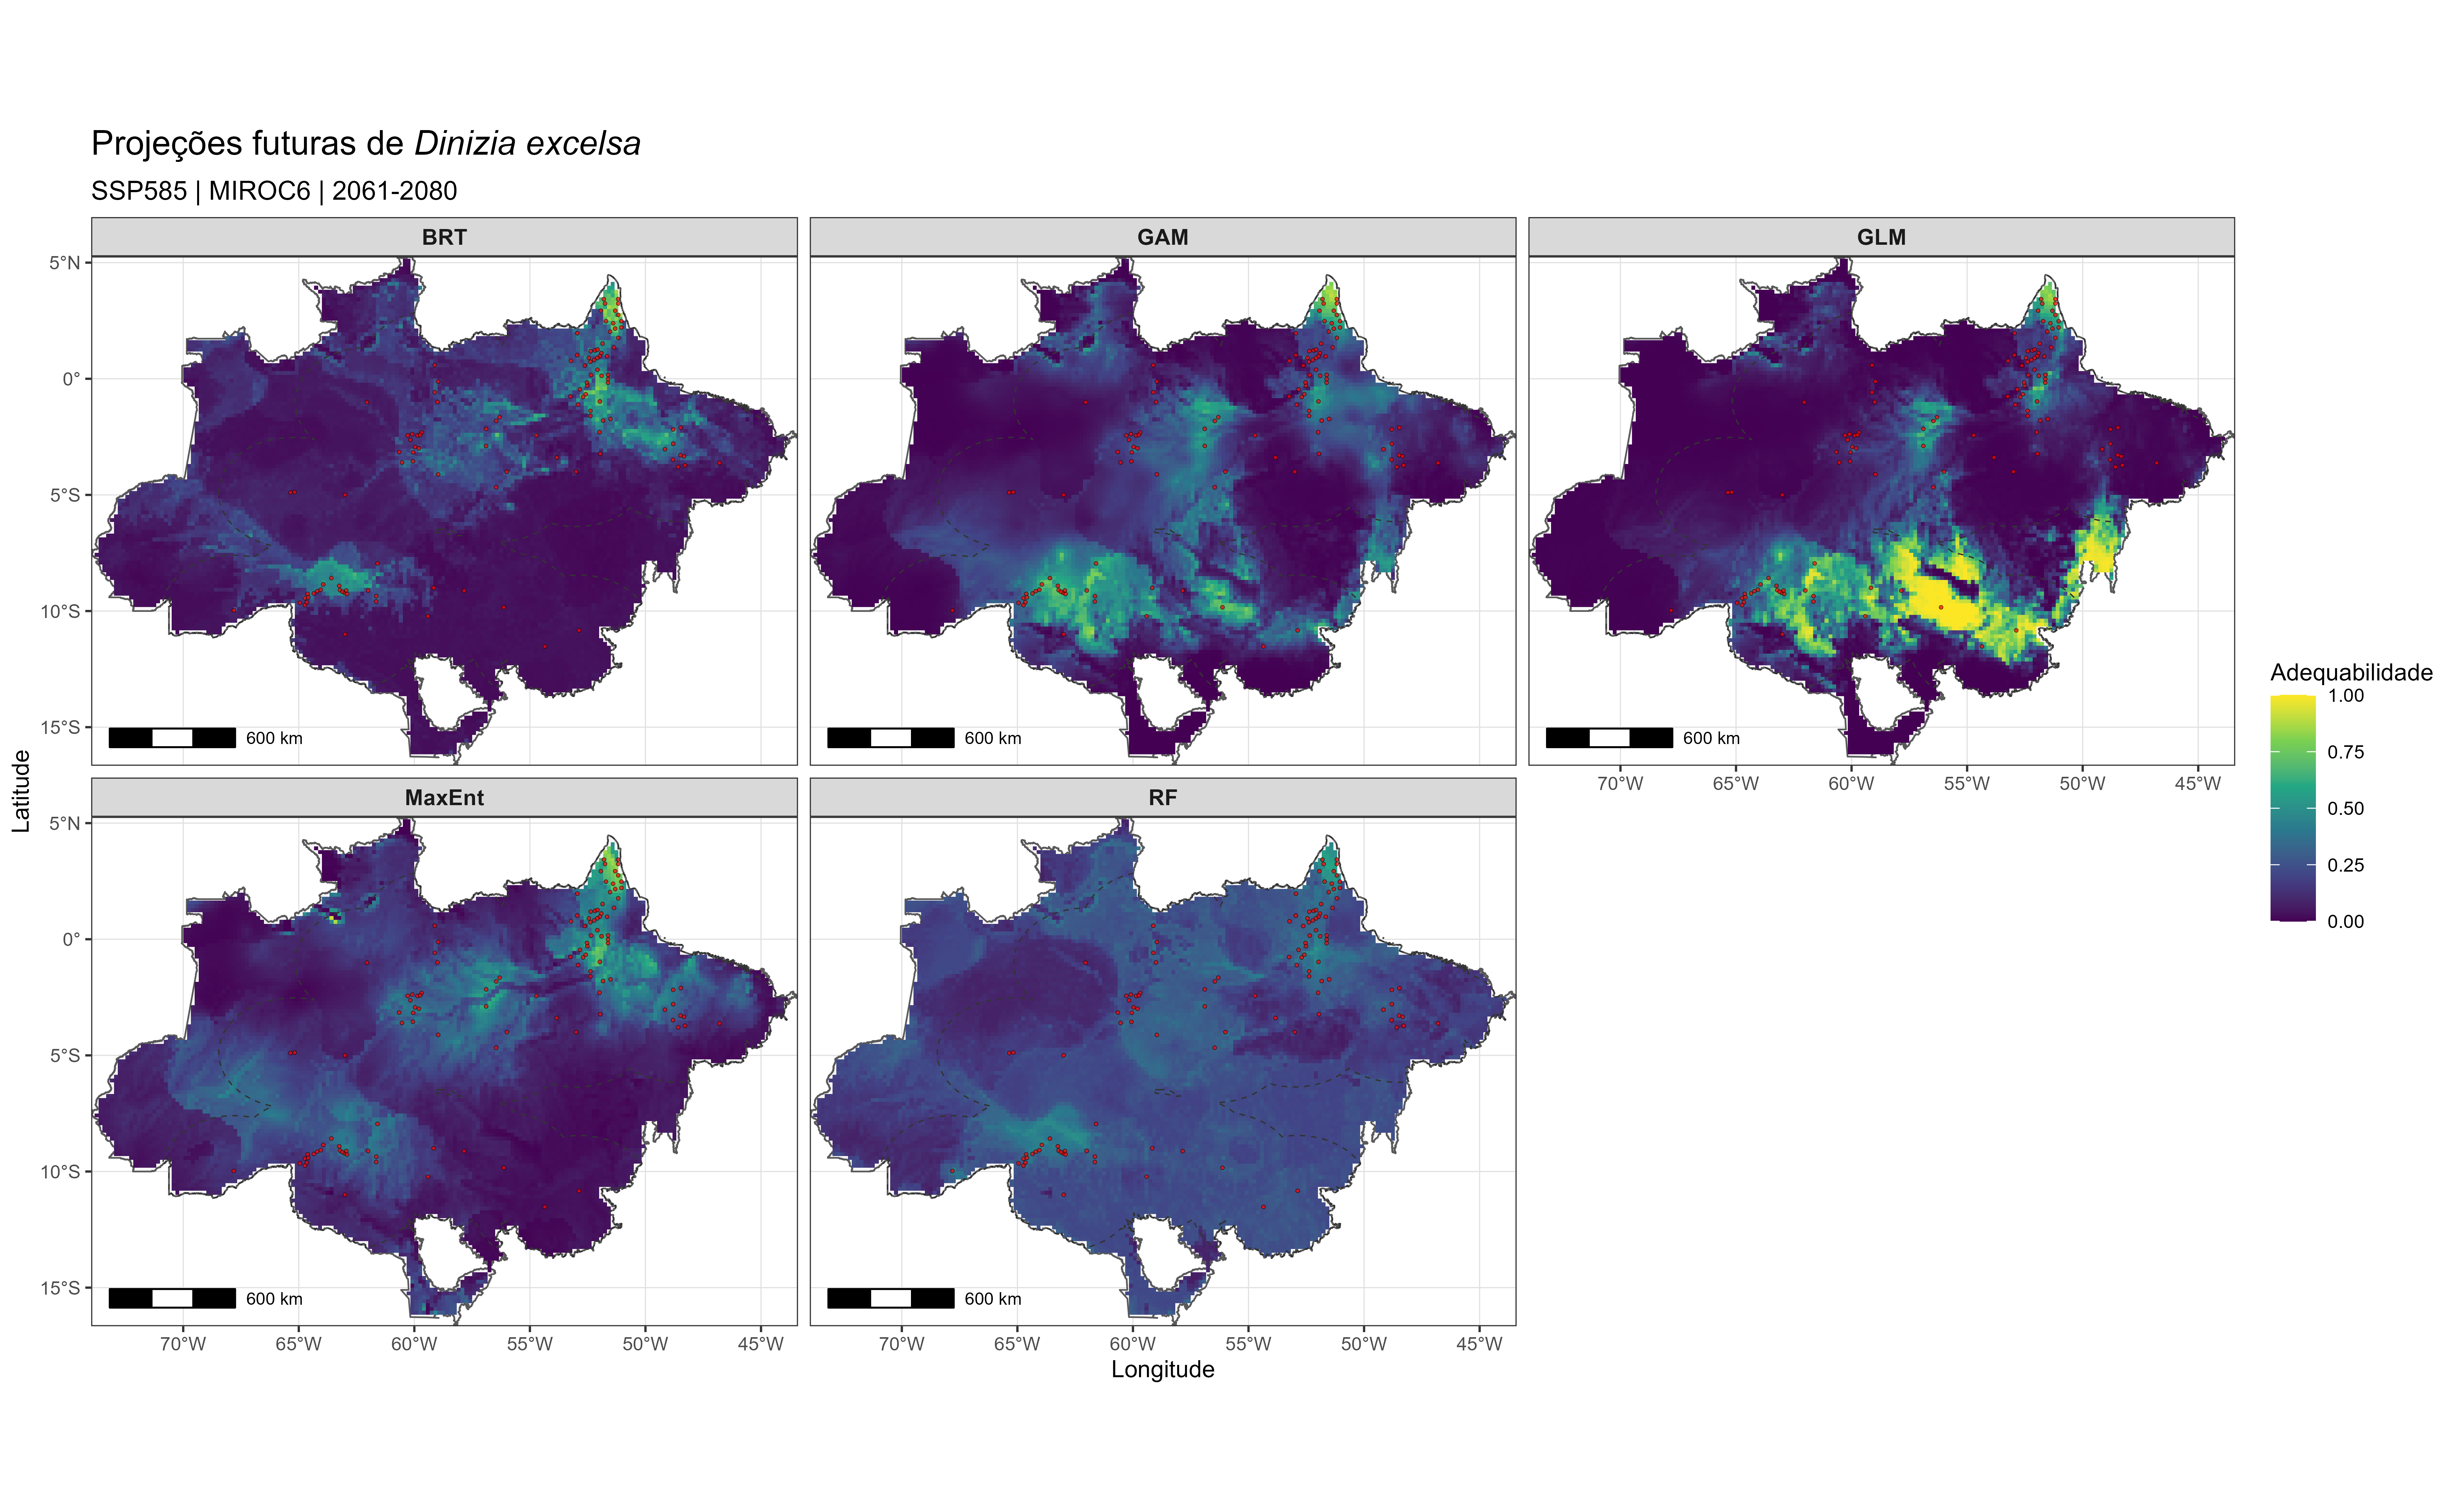
\includegraphics[width=0.98\textwidth]{figuras/unidade13/unidade13_modelos_futuros_ssp585.png}
	\caption{Projeções futuras dos modelos individuais para \textit{Dinizia excelsa} sob cenário SSP585.}
	\label{fig:unidade13_modelos_futuros}
\end{figure}

\section{Ensemble futuro}

As projeções individuais são combinadas para gerar mapas ensemble futuros por cenário. O ensemble reduz a dependência de um único algoritmo e permite comparar padrões médios de adequabilidade entre cenários.

\rscriptfile{scripts/unidade13/04_ensemble_futuro.R}

\begin{figure}[H]
	\centering
	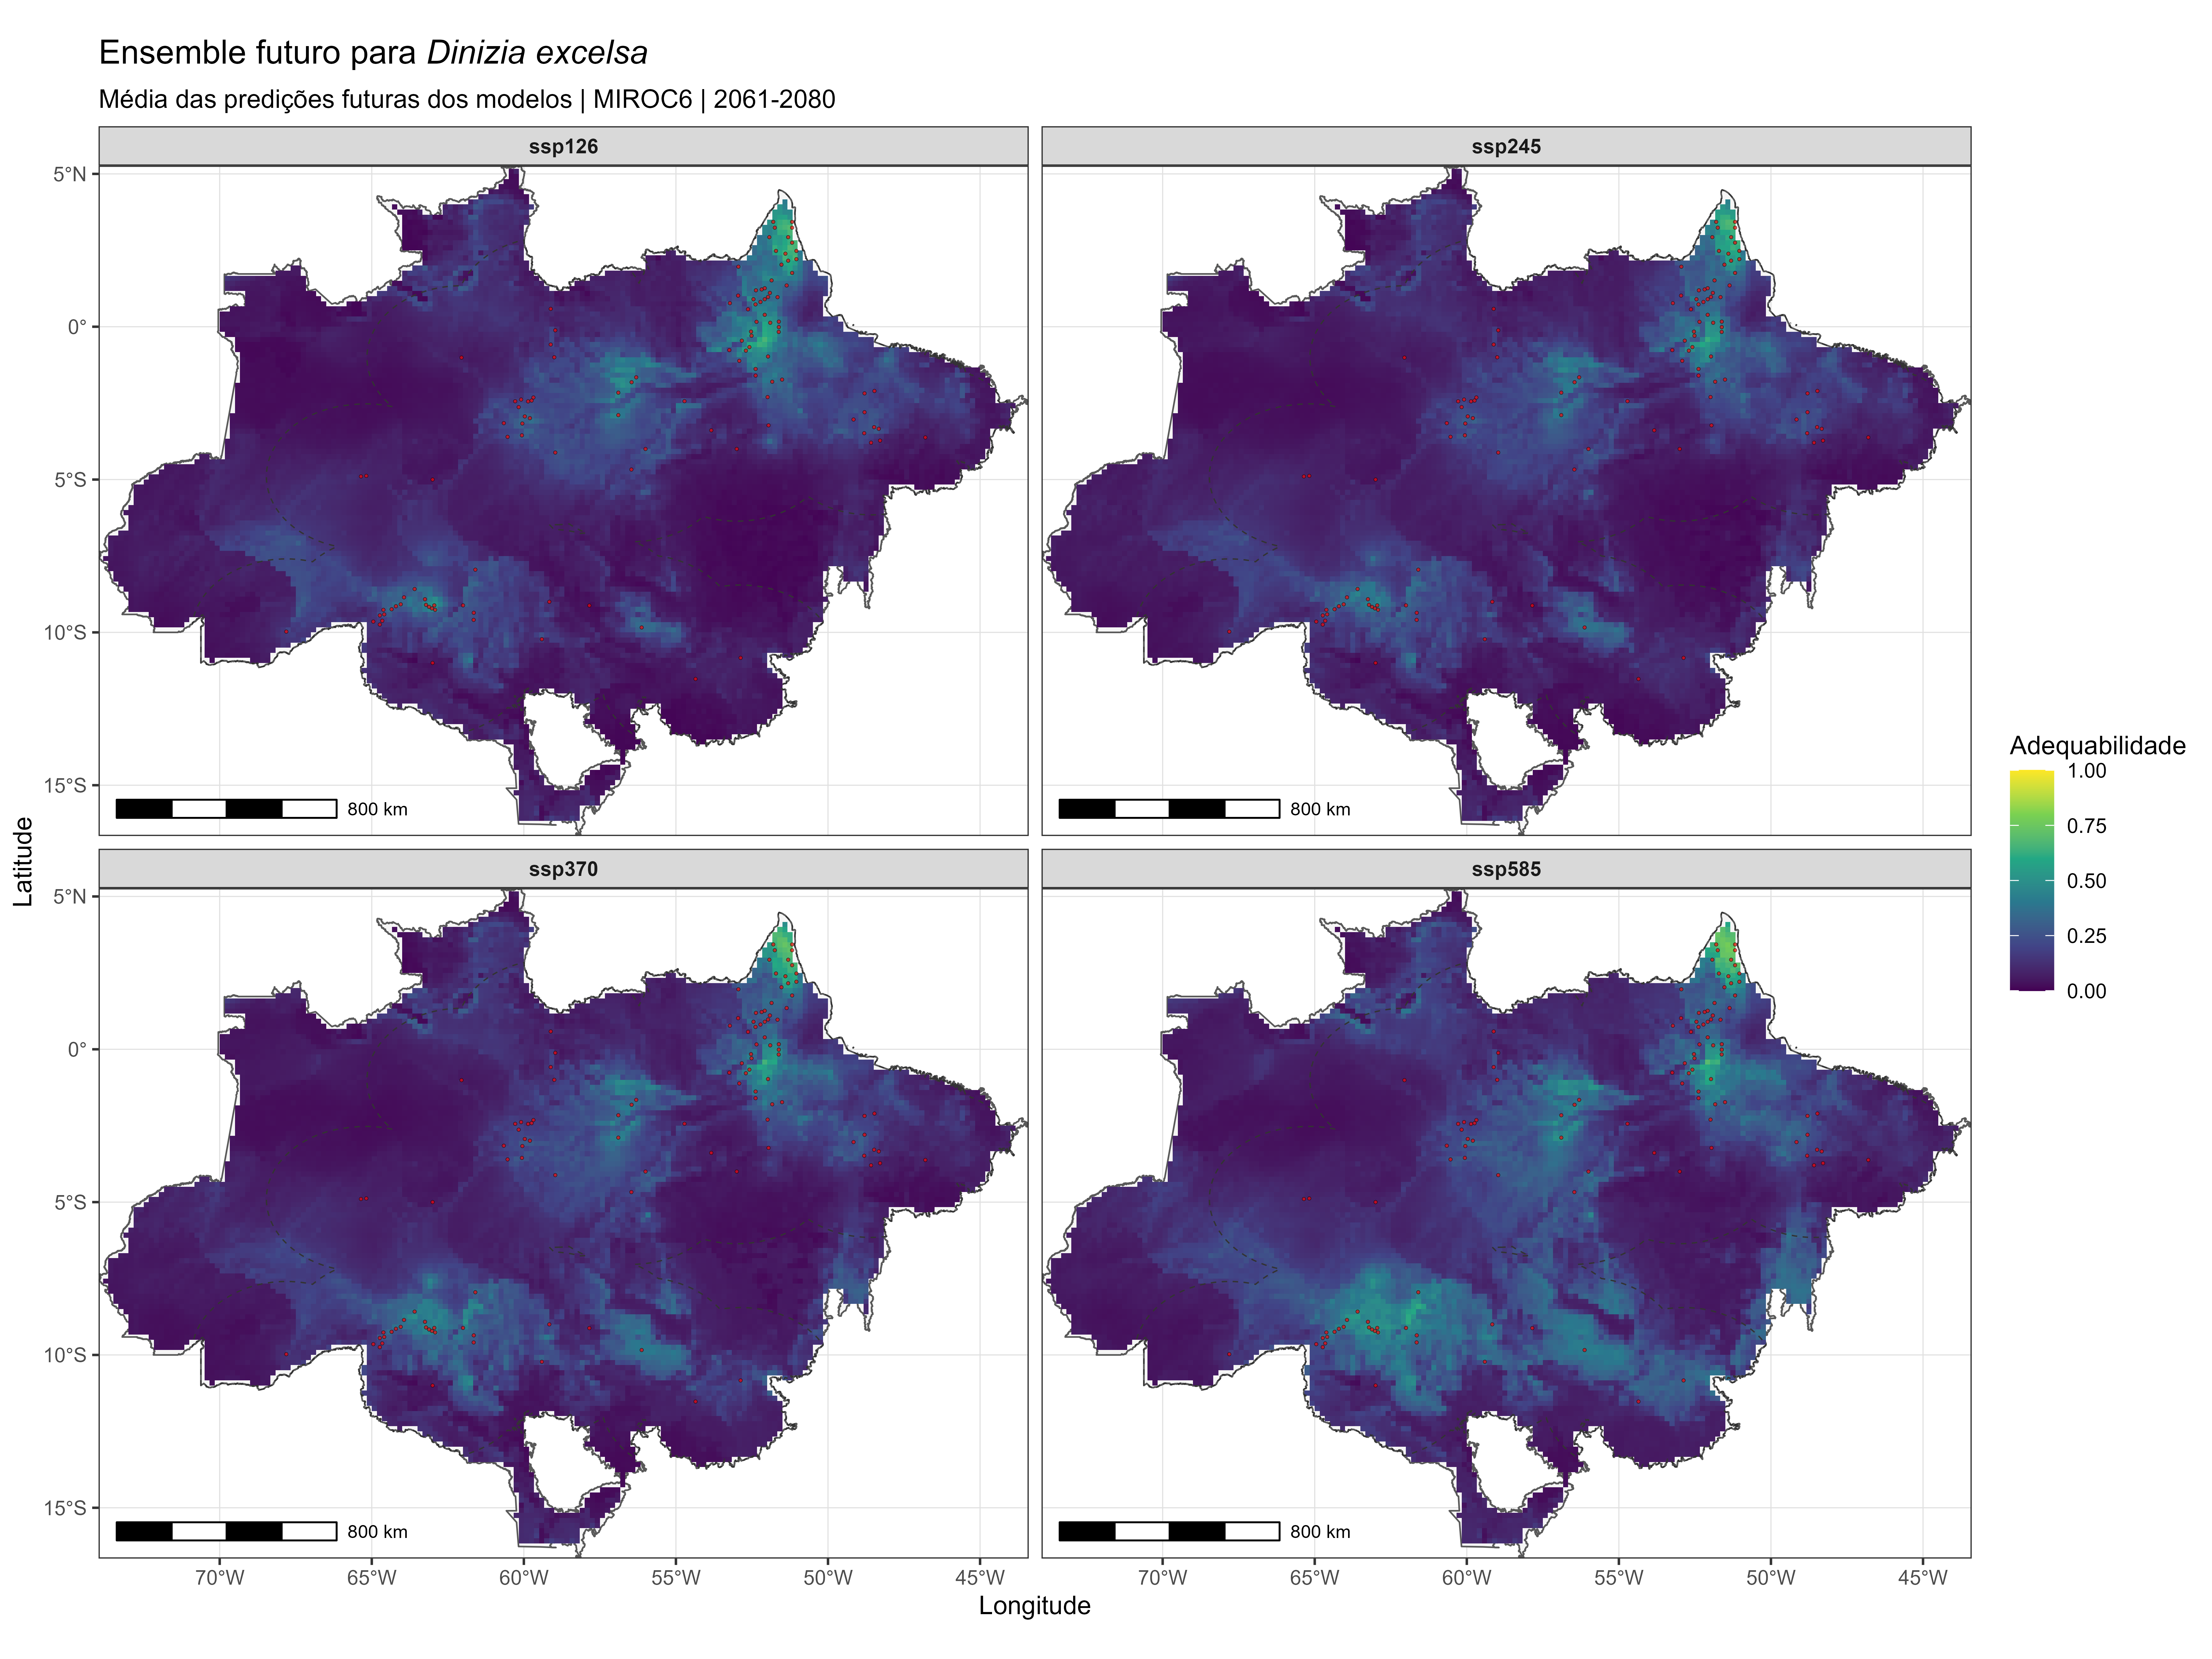
\includegraphics[width=0.96\textwidth]{figuras/unidade13/unidade13_ensemble_futuro_cenarios.png}
	\caption{Mapas ensemble futuros de adequabilidade ambiental de \textit{Dinizia excelsa} sob diferentes cenários SSP.}
	\label{fig:unidade13_ensemble_futuro}
\end{figure}

\section{Mudança de adequabilidade}

A mudança de adequabilidade é calculada pela diferença entre a adequabilidade futura e a adequabilidade atual. Valores positivos indicam aumento relativo de adequabilidade; valores negativos indicam redução.

\begin{equationbox}
	\[
	\Delta S = S_{futuro} - S_{atual}
	\]
\end{equationbox}

em que \(S_{futuro}\) é a adequabilidade projetada para um cenário futuro e \(S_{atual}\) é a adequabilidade estimada no período atual.

\rscriptfile{scripts/unidade13/05_mudanca_adequabilidade.R}

\begin{figure}[H]
	\centering
	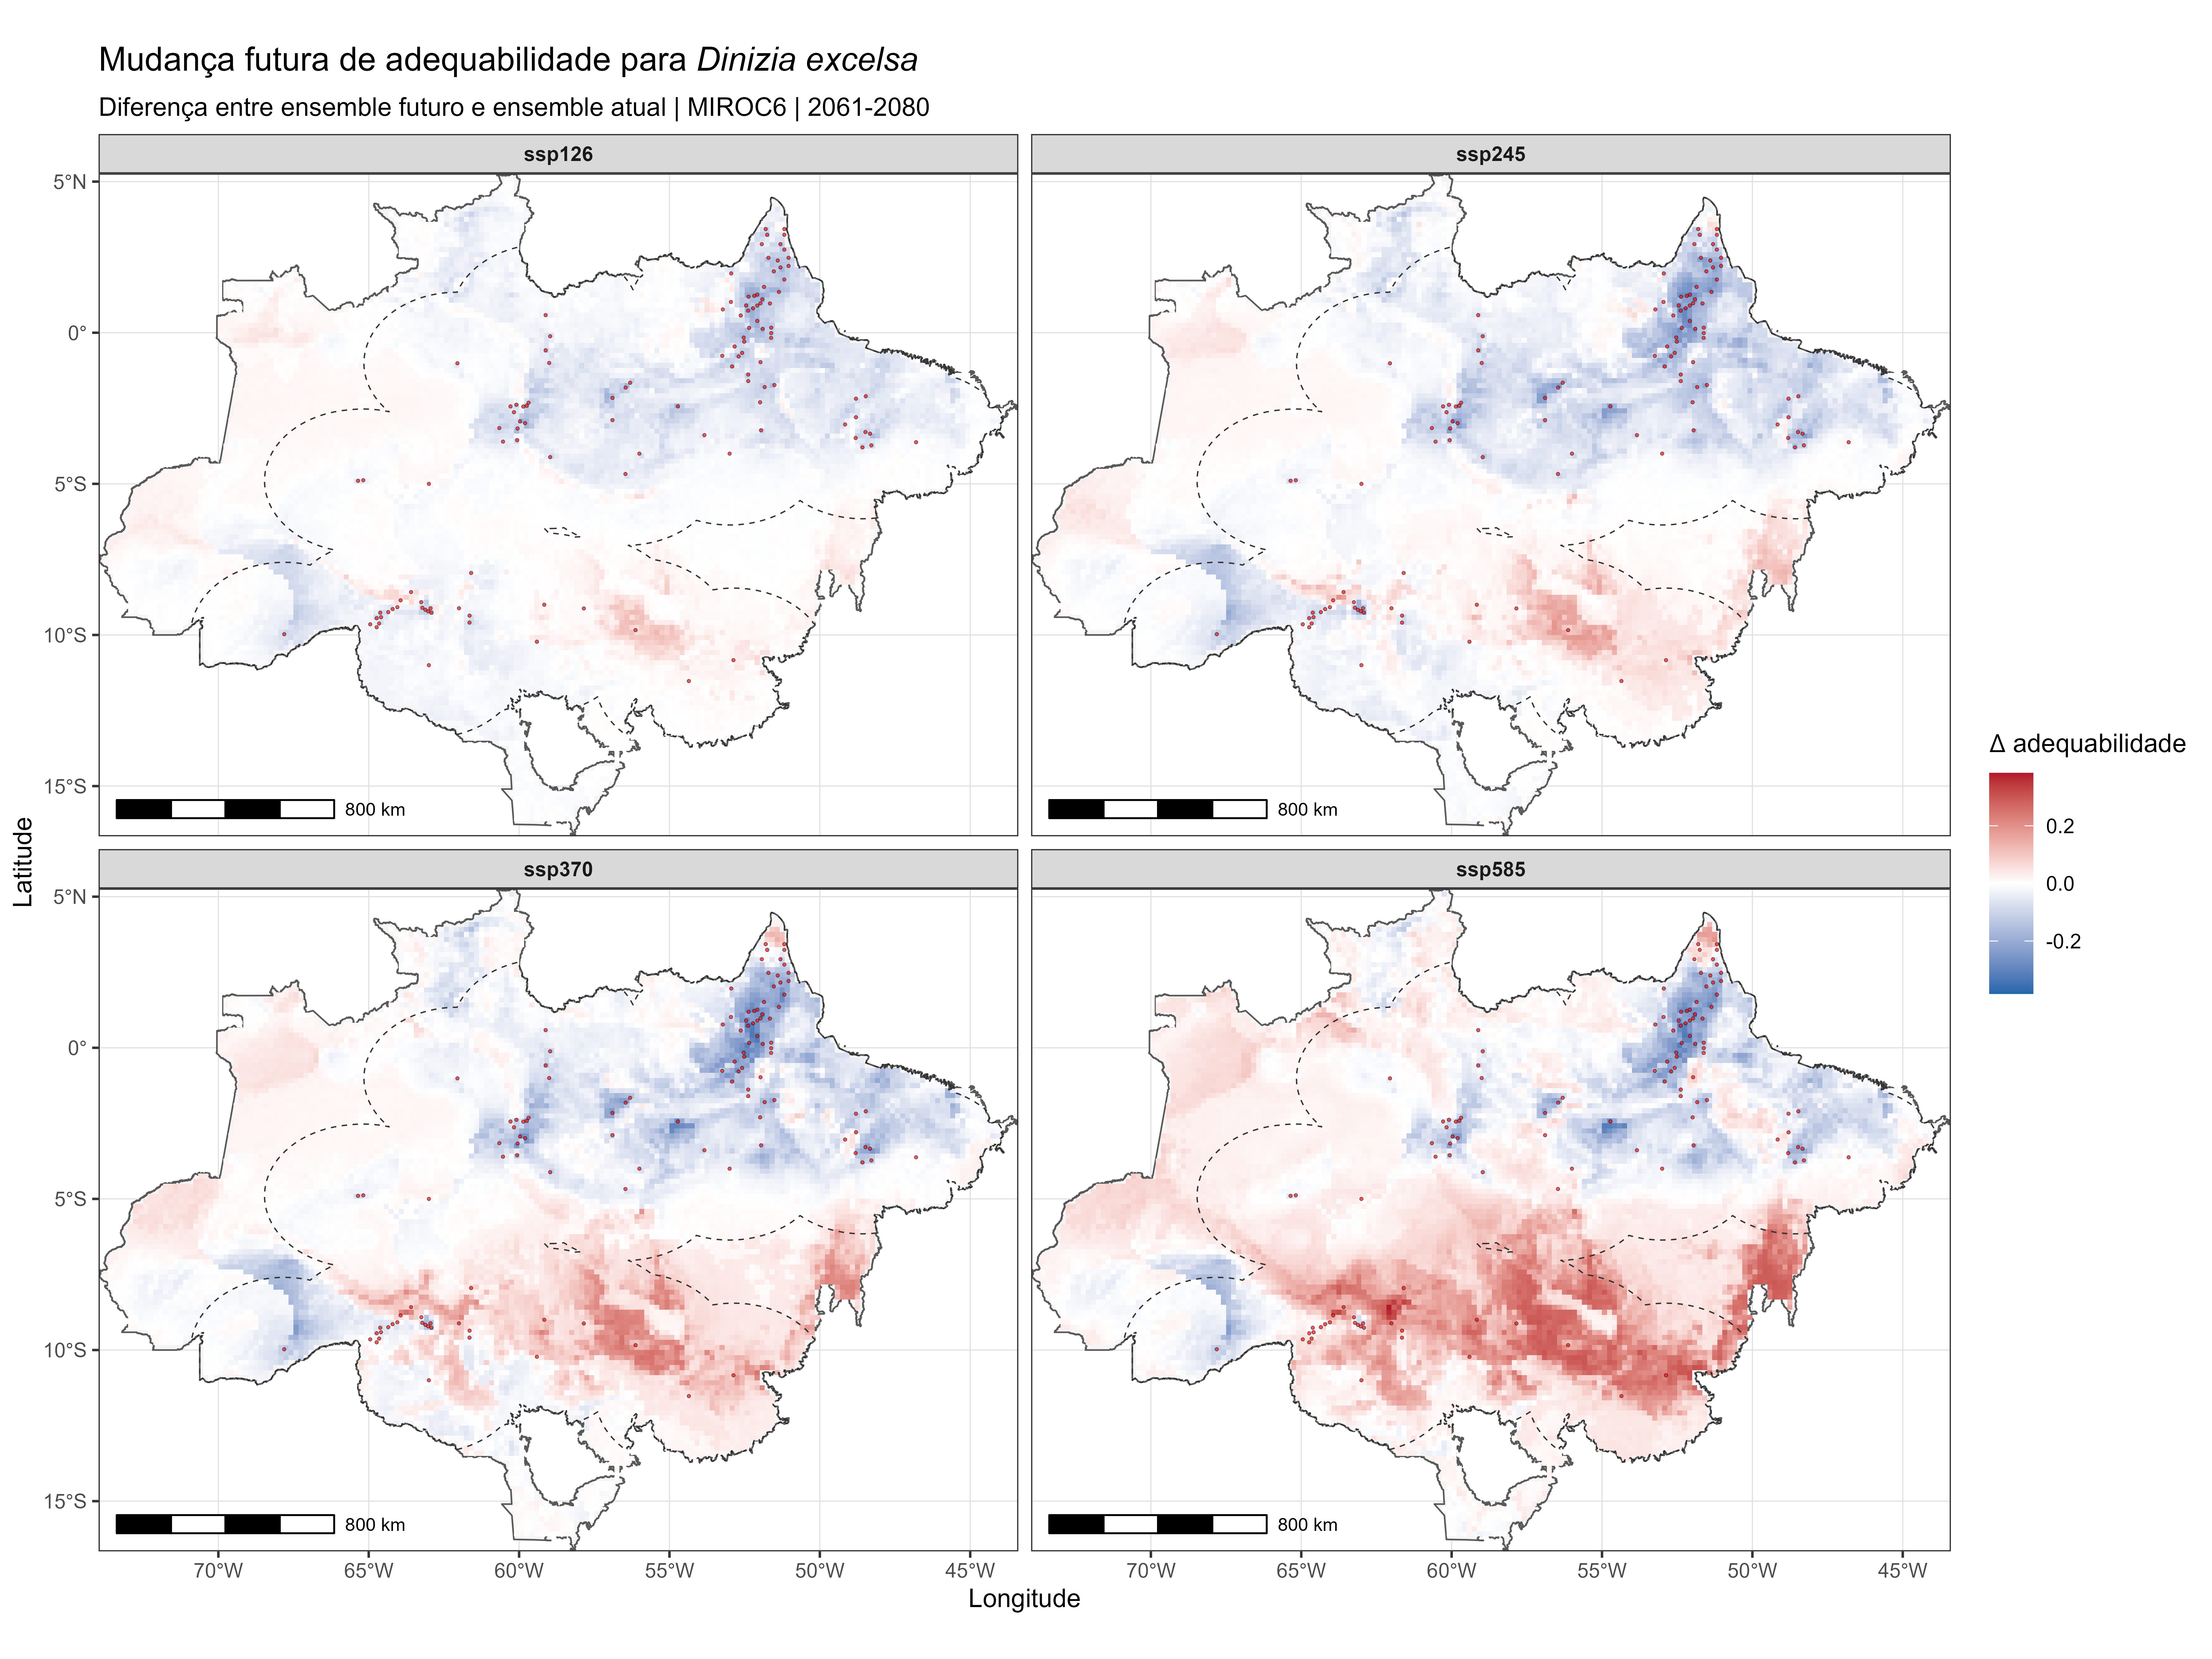
\includegraphics[width=0.96\textwidth]{figuras/unidade13/unidade13_mudanca_adequabilidade.png}
	\caption{Mudança de adequabilidade ambiental futura em relação ao cenário atual para \textit{Dinizia excelsa}.}
	\label{fig:unidade13_mudanca}
\end{figure}

\section{Áreas estáveis, perdas e ganhos}

A comparação entre mapas binários atuais e futuros permite classificar as células em áreas estáveis, áreas de perda potencial, áreas de ganho potencial e áreas persistentemente inadequadas.

\rscriptfile{scripts/unidade13/06_estabilidade_perda_ganho.R}

\begin{figure}[H]
	\centering
	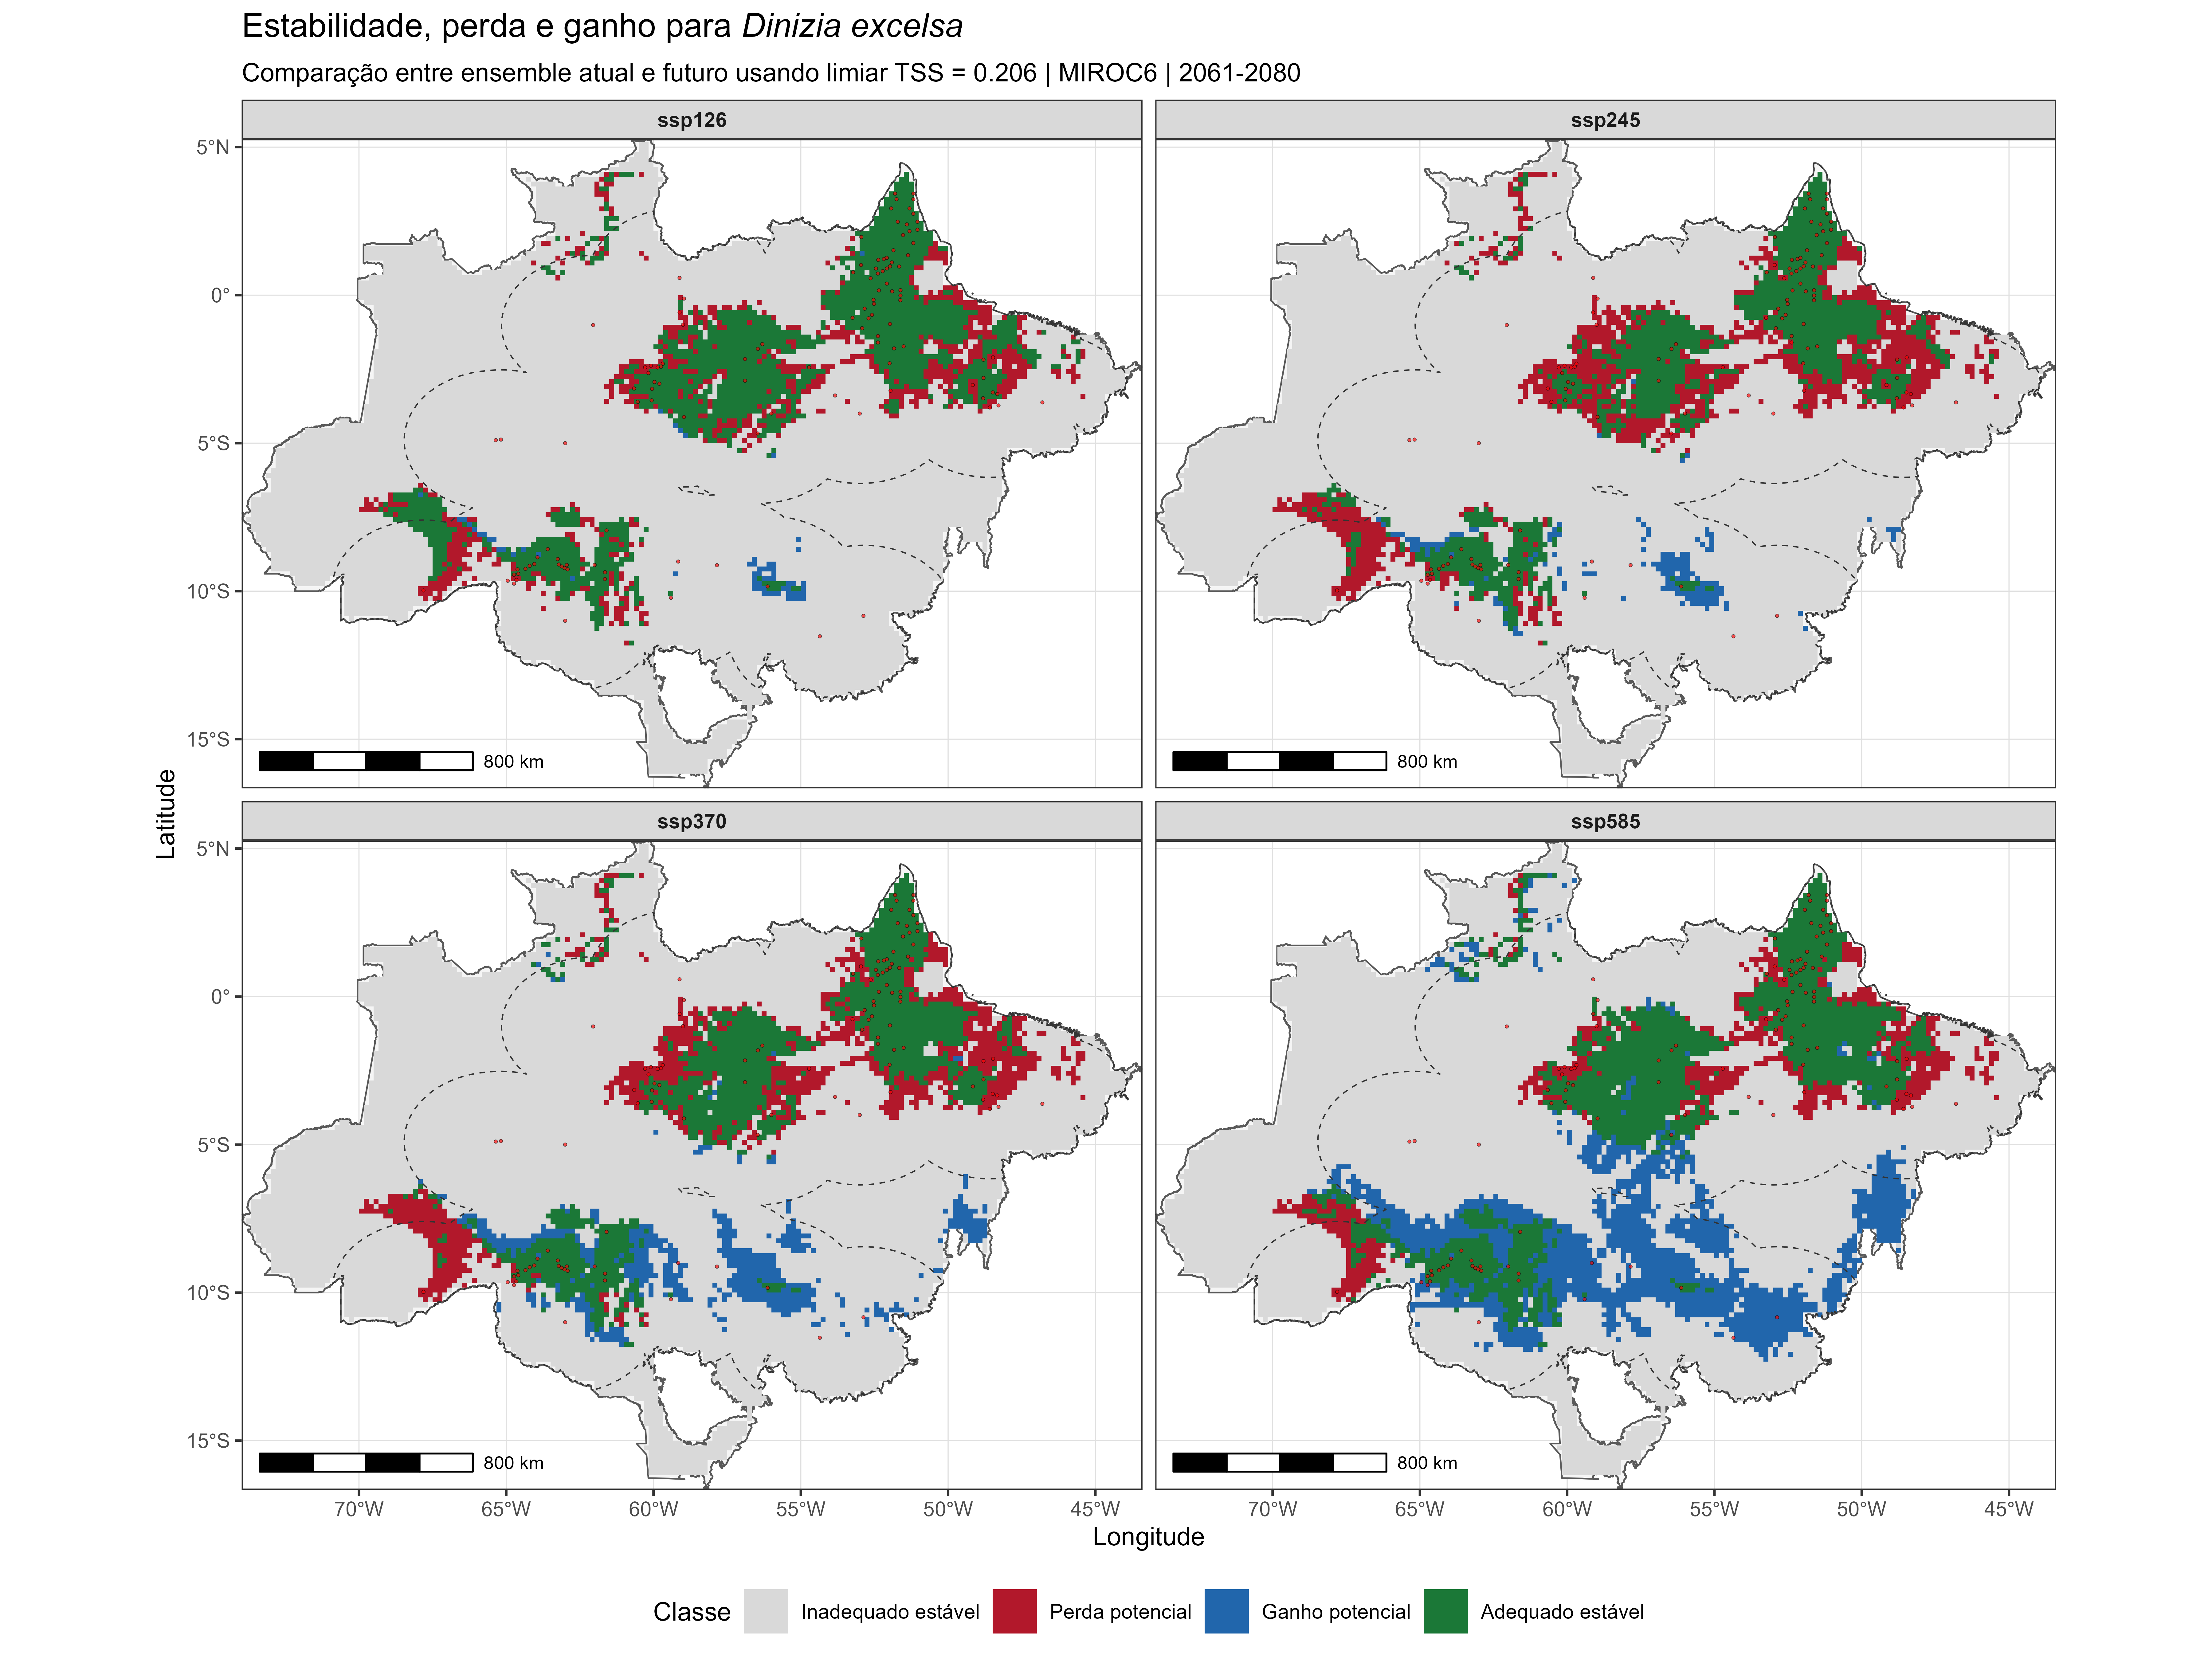
\includegraphics[width=0.96\textwidth]{figuras/unidade13/unidade13_estabilidade_perda_ganho.png}
	\caption{Áreas de estabilidade, perda e ganho potencial de adequabilidade ambiental para \textit{Dinizia excelsa} sob cenários futuros.}
	\label{fig:unidade13_estabilidade}
\end{figure}

\section{Síntese tabular dos cenários}

\rscriptfile{scripts/unidade13/07_sintese_cenarios_futuros.R}

\begin{figure}[H]
	\centering
	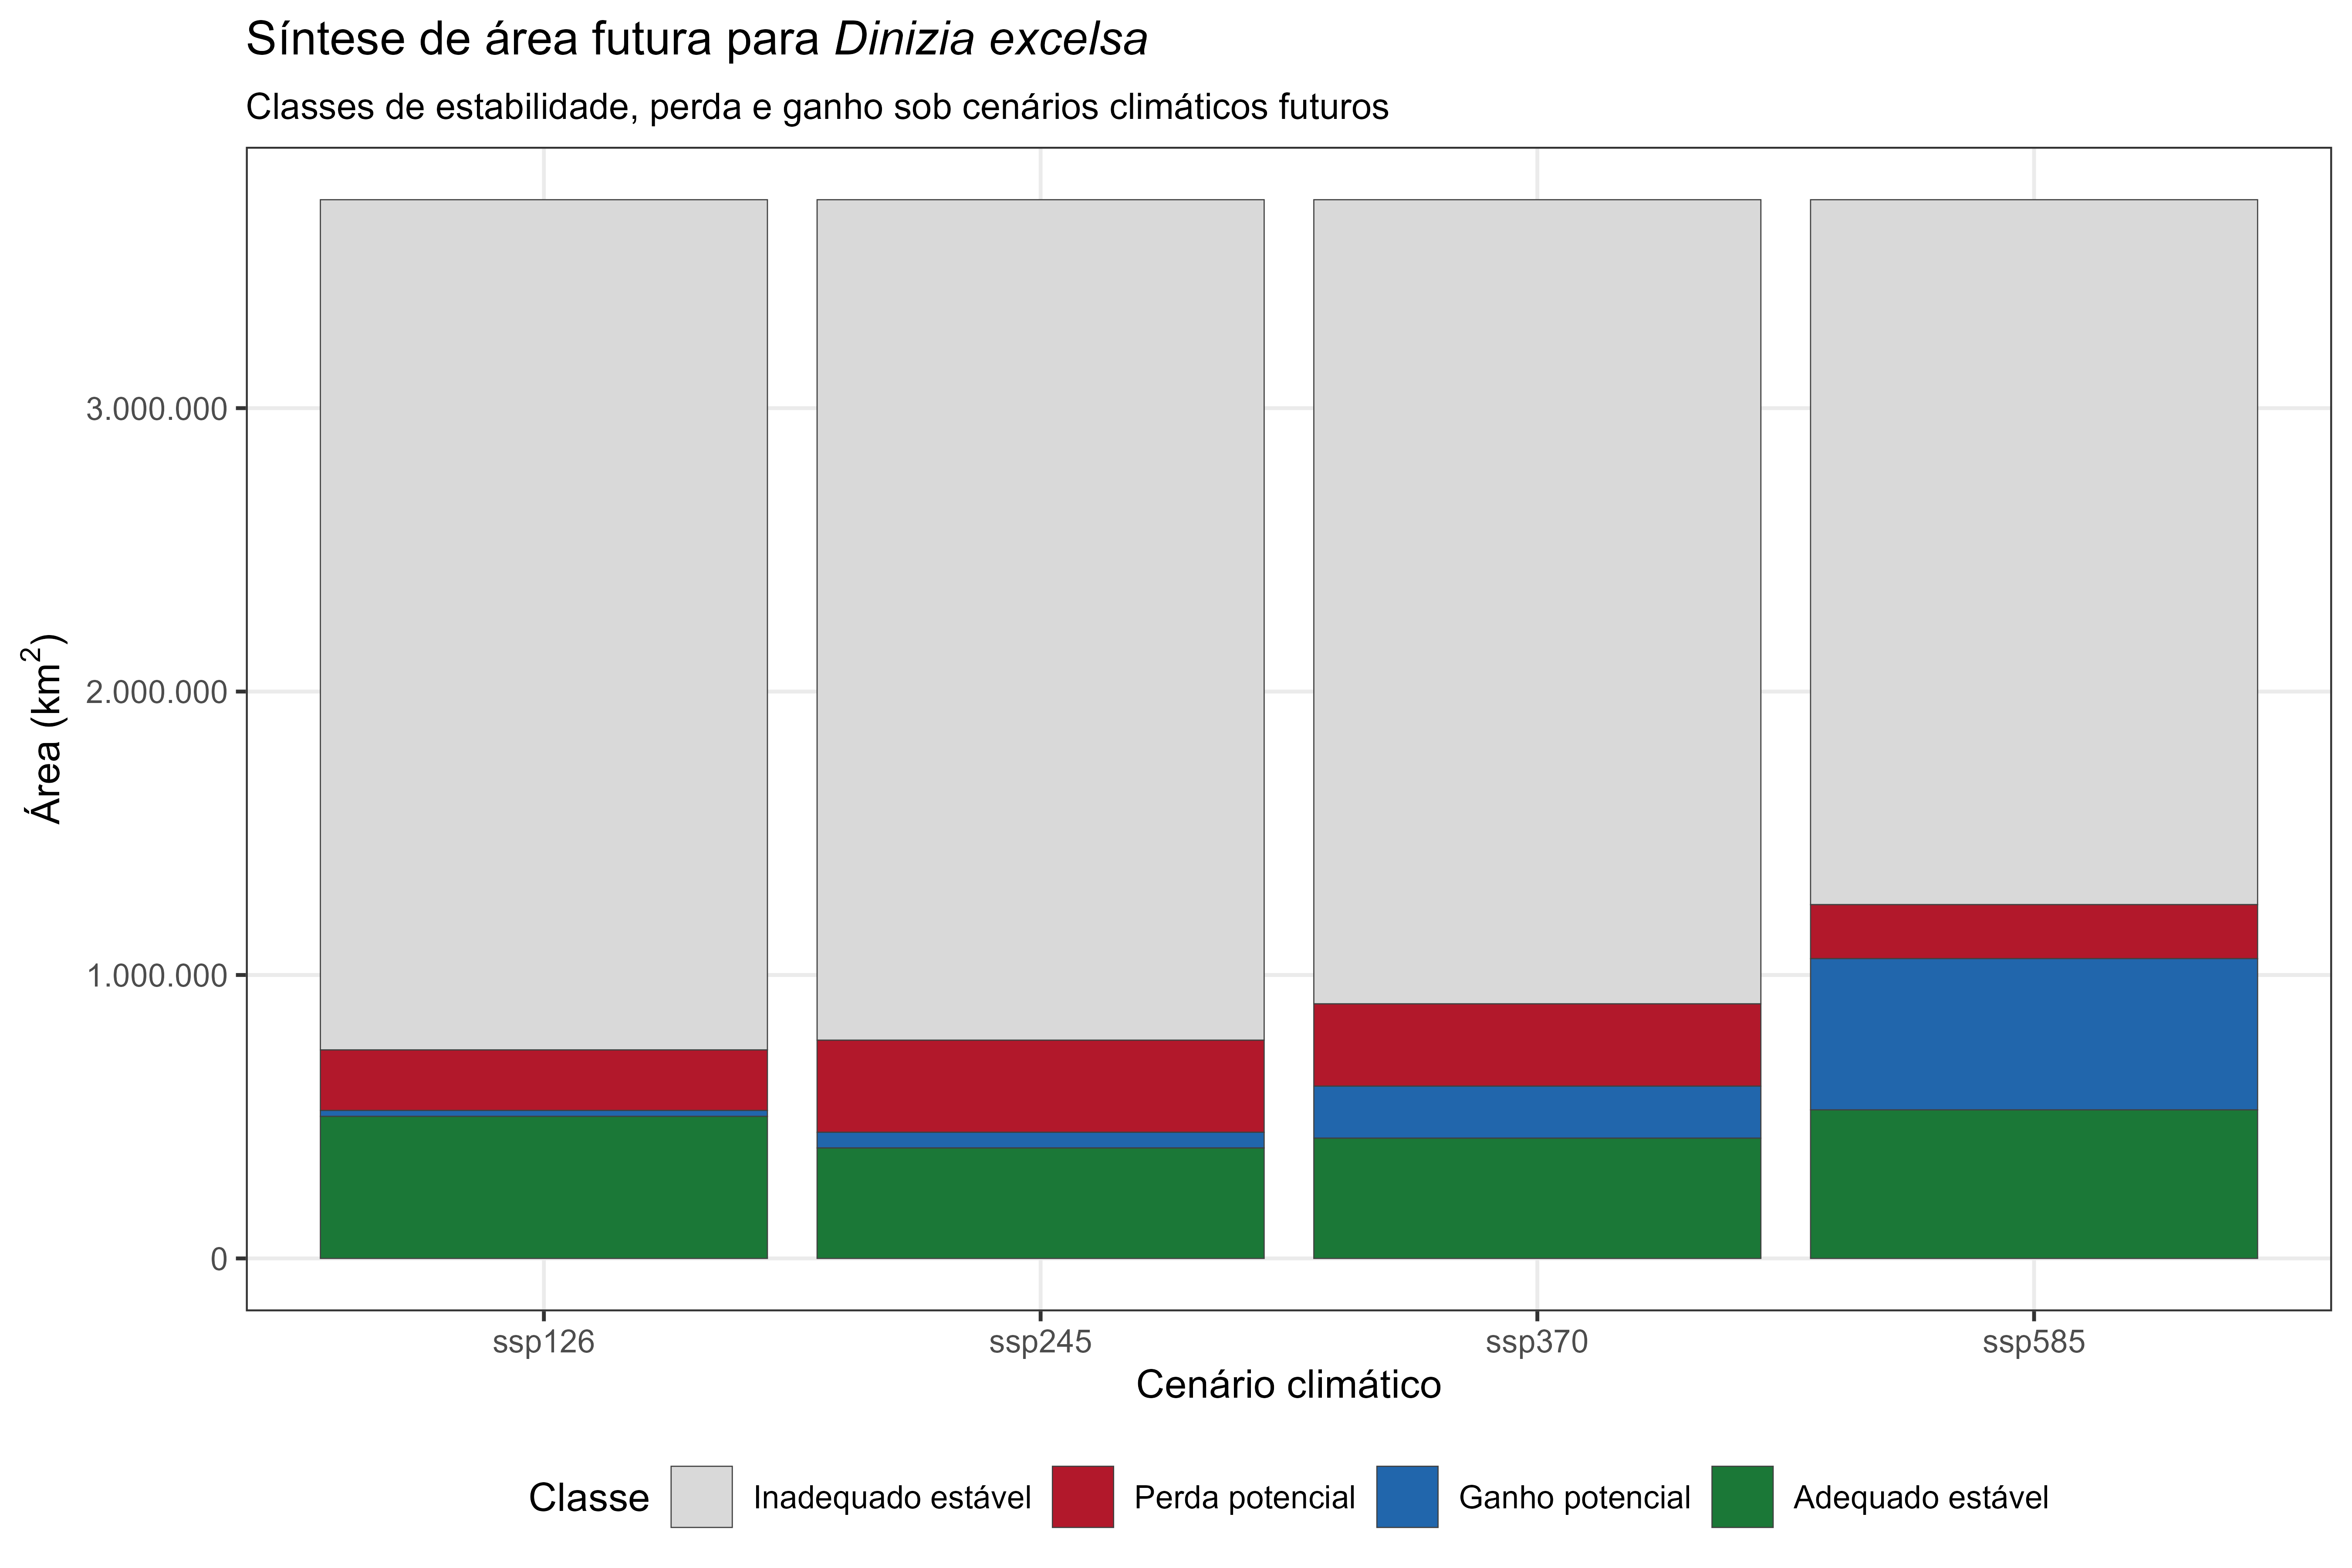
\includegraphics[width=0.88\textwidth]{figuras/unidade13/unidade13_sintese_area_adequada.png}
	\caption{Síntese da área potencialmente adequada atual e futura para \textit{Dinizia excelsa} sob diferentes cenários SSP.}
	\label{fig:unidade13_sintese_area}
\end{figure}

\section{Pipeline completo}

\rscriptfile{scripts/unidade13/08_pipeline_projecoes_futuras.R}

\section{Síntese da unidade}

As projeções climáticas futuras permitem avaliar possíveis mudanças na adequabilidade ambiental de espécies sob diferentes trajetórias climáticas. Para \textit{Dinizia excelsa}, esse tipo de análise é especialmente relevante para discutir persistência climática, áreas prioritárias, estabilidade ambiental e riscos associados a cenários de aquecimento.

\begin{conceito}[title={\faBook\quad Mensagem central}]
	Projeções futuras em SDM devem ser interpretadas como cenários de adequabilidade ambiental, não como previsões determinísticas de ocorrência. A robustez da interpretação depende da qualidade dos dados atuais, da escolha dos cenários, da compatibilidade das variáveis e da avaliação das incertezas.
\end{conceito}

\section{Exercícios de fixação}

\begin{enumerate}
	\item Explique a diferença entre clima atual e clima futuro em SDM.
	\item O que são cenários SSP?
	\item Por que as variáveis futuras devem ter os mesmos nomes das variáveis usadas no ajuste atual?
	\item Como interpretar valores positivos e negativos de mudança de adequabilidade?
	\item O que são áreas de estabilidade climática?
	\item Por que projeções futuras não devem ser interpretadas como previsões absolutas?
	\item Como os resultados desta unidade podem apoiar decisões de conservação?
\end{enumerate}

% ============================================================
% UNIDADE 14
% ============================================================

